\documentclass[UTF8,a4paper,11pt]{ctexart}

% ── Page geometry ──
\usepackage[margin=2.2cm,top=2.5cm,bottom=2.5cm]{geometry}

% ── Typography & math ──
\usepackage{fontspec}
\usepackage{amsmath,amssymb}
\usepackage{setspace}
\setstretch{1.25}

% ── Graphics ──
\usepackage{tikz}
\usetikzlibrary{arrows.meta,calc}

% ── Colors ──
\usepackage{xcolor}
\definecolor{accent}{HTML}{1a73e8}
\definecolor{darkgray}{HTML}{333333}
\definecolor{lightgray}{HTML}{f5f5f5}
\definecolor{notebg}{HTML}{e8f0fe}
\definecolor{warnbg}{HTML}{fef7e0}
\definecolor{calcbg}{HTML}{e6f4ea}
\definecolor{calcframe}{HTML}{188038}

% ── Links ──
\usepackage{hyperref}
\hypersetup{colorlinks=true,linkcolor=accent,urlcolor=accent}

% ── Layout ──
\usepackage{enumitem}
\setlist[itemize]{leftmargin=1.8em,itemsep=2pt}
\setlist[enumerate]{leftmargin=1.8em,itemsep=2pt}
\usepackage{booktabs}
\usepackage{tcolorbox}
\usepackage{titlesec}
\usepackage{fancyhdr}
\usepackage{lastpage}

% ── Header/Footer ──
\pagestyle{fancy}
\fancyhf{}
\fancyhead[L]{\small\textcolor{darkgray}{高中物理必修一 · 七天核心概念讲义}}
\fancyhead[R]{\small\textcolor{darkgray}{从第一性原理理解运动与力}}
\fancyfoot[C]{\small\textcolor{darkgray}{\thepage\ / \pageref{LastPage}}}
\renewcommand{\headrulewidth}{0.4pt}

% ── Section styling ──
\titleformat{\section}
  {\Large\bfseries\color{accent}}
  {\thesection}{1em}{}
\titleformat{\subsection}
  {\large\bfseries\color{darkgray}}
  {\thesubsection}{1em}{}

% ── Custom boxes ──
\newtcolorbox{keyconcept}[1][]{
  colback=notebg, colframe=accent,
  fonttitle=\bfseries, boxrule=0.5pt,
  left=8pt, right=8pt, top=6pt, bottom=6pt, title={#1}}
\newtcolorbox{exercise}[1][]{
  colback=warnbg, colframe=orange,
  fonttitle=\bfseries, boxrule=0.5pt,
  left=8pt, right=8pt, top=6pt, bottom=6pt, title={#1}}
\newtcolorbox{calcbox}[1][]{
  colback=calcbg, colframe=calcframe,
  fonttitle=\bfseries, boxrule=0.5pt,
  left=8pt, right=8pt, top=6pt, bottom=6pt, title={#1}}

\newcommand{\daytitle}[2]{%
  \section*{#1\quad #2}%
  \addcontentsline{toc}{section}{#1\quad #2}}

\begin{document}

% ═══ 封面 ═══
\begin{center}
  \vspace*{2cm}
  {\Huge\bfseries\color{accent} 高中物理必修一}\\[0.4cm]
  {\LARGE 七天核心概念讲义}\\[1.2cm]
  {\large 写给准高中生：从第一性原理理解运动与力}\\[0.5cm]
  {\small\textcolor{darkgray}{依据：普通高中教科书《物理》必修第一册（沪科版）}}\\[0.3cm]
  {\small\textcolor{darkgray}{\today}}
  \vfill
  {\small 每天 60–90 分钟：先读讲解，再合上讲义把概念讲出来，最后做自测。}
\end{center}
\newpage

\tableofcontents
\newpage

% ═══ 使用说明 ═══
\section*{开始前：这本讲义在做什么}
\addcontentsline{toc}{section}{开始前：这本讲义在做什么}

必修一这本书，其实只回答两个问题：

\begin{enumerate}
  \item \textbf{怎样精确地描述运动？}（第一、二章：位移、速度、加速度、匀变速直线运动）
  \item \textbf{运动为什么会改变？}（第三、四章：力、力的合成与分解、牛顿运动定律）
\end{enumerate}

它在初中物理之上，真正新增的只有三样工具：

\begin{keyconcept}[一周要带走的三样工具]
\begin{itemize}
  \item \textbf{矢量}：有方向的量。位移、速度、加速度、力都是矢量。初中只处理一条直线上的加减，高中要处理任意方向——合成与分解。
  \item \textbf{变化率}（微积分的直觉）：速度是位置的变化率，加速度是速度的变化率。“瞬时”两个字背后就是极限思想，这是高中物理和初中物理最大的分水岭。
  \item \textbf{牛顿第二定律 $F_{\text{合}}=ma$}：把“力”和“运动”焊在一起的方程。整部必修一就是为了让你真正理解这一个等式。
\end{itemize}
\end{keyconcept}

\textbf{每天的学习流程}（60–90 分钟）：
\begin{enumerate}
  \item 读当天的讲解，重点看“为什么这样定义”，不要背结论；
  \item 合上讲义，把当天的核心概念\textbf{讲给别人听}（或讲给自己听），卡壳的地方就是没懂的地方；
  \item 做“今日自测”，对照书末的答案。
\end{enumerate}

\newpage

% ═══ 第 1 天 ═══
\daytitle{第 1 天}{物理学的第一课：先学会“忽略”}

\textbf{核心问题}：怎样精确地说清一个物体在哪里、往哪去？

\subsection*{1.1 质点：不是“很小”，而是“不重要”}

你想描述一列从北京开往上海的高铁。它需要 4 个多小时、跑 1300 多公里——这时候，列车 200 米的车身长度重要吗？完全可以忽略。但同一列车进站停靠时，车门对准站台屏蔽门，车身长度就是全部问题的关键。

\begin{keyconcept}[质点与物理模型]
在某些情况下，可以忽略物体的大小和形状，把它抽象为一个有质量的点，这样的点称为\textbf{质点}。

判断标准从来不是物体本身的大小，而是\textbf{在这个问题里}，大小和形状是否影响答案。地球直径一万多千米，研究公转时它是质点；研究昼夜交替时它不是。
\end{keyconcept}

这是物理学最重要的思维方式：\textbf{物理学从不研究“完整的真实”，只研究“够用的简化”}。地图不是领土，模型不是实物——但一个好模型能给出足够准的答案。后面每一天你都会看到这个思想：忽略空气阻力、忽略摩擦、把力看成作用在一个点上……先决定忽略什么，才能开始计算。

\subsection*{1.2 参考系与位置}

“火车在动”这句话其实不完整——相对于站台它在动，相对于车厢里的乘客它没动。\textbf{描述任何运动，都要先说清楚相对于谁}，这个“谁”就是参考系。初中你已经用过它，高中只强调一件事：先选参考系，再谈运动。

选定参考系后，沿运动方向建一条数轴，物体的位置就是一个坐标 $x$（单位：米）。

\subsection*{1.3 位移：本讲义的第一个矢量}

从家到学校，你可以走直线，也可以绕公园一圈。轨迹长度不同，但“位置的变化”完全一样。物理学要精确区分这两件事：

\begin{keyconcept}[位移 vs 路程]
\begin{itemize}
  \item \textbf{位移} $\Delta x = x_2 - x_1$：从初位置指向末位置的\textbf{有向线段}。有大小、有方向——是\textbf{矢量}。
  \item \textbf{路程}：实际轨迹的长度。只有大小——是\textbf{标量}。
  \item 关系：路程 $\geq$ 位移的大小（只有单向直线运动时取等号）。
\end{itemize}
\end{keyconcept}

\begin{center}
\begin{tikzpicture}[>=Stealth,scale=1.05]
  \fill (0,0) circle (1.8pt) node[below left] {A（起点）};
  \fill (5.2,1.6) circle (1.8pt) node[above right] {B（终点）};
  \draw[thick,darkgray] (0,0) .. controls (1.5,2.4) and (3.5,-0.8) .. (5.2,1.6);
  \node[darkgray] at (2.9,1.9) {路程（实际轨迹的长度）};
  \draw[->,very thick,accent] (0,0) -- (5.2,1.6);
  \node[accent] at (2.4,-0.55) {位移 $\Delta x$：由 A 指向 B 的有向线段};
\end{tikzpicture}
\end{center}

负号的意义：规定向右为正方向，$\Delta x = -3$ 米不是说“位置变化变少了”，而是说\textbf{位移大小 3 米、方向向左}。矢量的正负号只表示方向，不表示大小。

\begin{exercise}[今日自测]
\begin{enumerate}
  \item 研究地球公转时可以把地球看作质点，研究地球自转时也可以吗？为什么？
  \item 你绕 400 米操场跑了一圈回到起点。路程是多少？位移是多少？
  \item 一人先向东走 4 米，再向西走 3 米。位移是多少（以向东为正）？路程是多少？
\end{enumerate}
\end{exercise}

\newpage

% ═══ 第 2 天 ═══
\daytitle{第 2 天}{快慢的精确化：从平均速度到瞬时速度}

\textbf{核心问题}：汽车速度表上的 80 km/h，到底是什么意思？

\subsection*{2.1 平均速度：一段时间的整体表现}

初中的 $v = \dfrac{s}{t}$ 其实藏了一个没说破的前提：它描述的是\textbf{整段过程}的平均快慢。高中把它写得更精确：

\[
\bar{v} = \frac{\Delta x}{\Delta t}
\]

注意分子是\textbf{位移}，不是路程。$\bar{v}$ 是矢量，方向与位移相同。如果把分子换成长度（路程），得到的叫\textbf{平均速率}，是标量。绕操场跑一圈回到起点：平均速度为 0（位移为 0），平均速率不为 0——这两个量的区别第一天就埋下了。

\subsection*{2.2 瞬时速度：一个时刻的速度}

但平均速度回答不了“速度表”的问题。车在这一瞬间跑多快？物理学家的办法是：\textbf{把“这一瞬间”逼近出来}——

测 10 秒内的平均速度，太粗；测 1 秒内，好一点；测 0.01 秒内……时间间隔 $\Delta t$ 越取越小，平均速度就越来越接近那个时刻的真实快慢。当 $\Delta t$ 小到趋近于 0 时，平均速度的极限值，就是\textbf{瞬时速度}：

\[
v = \lim_{\Delta t \to 0}\ \frac{\Delta x}{\Delta t}
\]

这不是玄学，实验室里就是这么测的：光电门配一片挡光片，挡光时间 $\Delta t$ 内片宽 $\Delta x$ 除以 $\Delta t$ 就是平均速度——\textbf{挡光片越窄，越接近瞬时速度}。

\begin{calcbox}[微积分初步（上）：极限与导数]
“令 $\Delta t$ 趋近于 0，看比值趋近于多少”，这个操作叫\textbf{取极限}，得到的结果叫\textbf{导数}。位置 $x$ 对时间 $t$ 的导数就是速度 $v$。

你现在不需要会算导数，只需要带走一个直觉：\textbf{“瞬时的量”都是某个比值在时间间隔无限缩小时的极限}。明天讲加速度，用的还是同一个思想。
\end{calcbox}

\subsection*{2.3 x–t 图像：斜率就是速度}

位置–时间图像（$x$ 纵轴、$t$ 横轴）把速度“画”了出来：

\begin{itemize}
  \item 图线上两点的连线（\textbf{割线}）的斜率 = 这段时间的\textbf{平均速度}；
  \item 图线上某点的\textbf{切线}斜率 = 该时刻的\textbf{瞬时速度}。
\end{itemize}

\begin{center}
\begin{tikzpicture}[>=Stealth,scale=1.5]
  \draw[->] (0,0) -- (3.9,0) node[right] {$t$};
  \draw[->] (0,0) -- (0,2.9) node[above] {$x$};
  % 曲线 x = 0.25 t^2
  \draw[very thick,accent] plot[domain=0:3.3,samples=40] (\x,{0.25*\x*\x});
  \node[accent] at (3.0,2.2) {$x(t)$};
  % 割线：t=1 到 t=2.5，斜率 0.875，过 (1,0.25)
  \draw[dashed,thick,darkgray] plot[domain=0.4:3.1] (\x,{0.875*(\x-1)+0.25});
  \node[darkgray] at (0.62,0.75) {割线};
  % 切线：t=1.6，斜率 0.8，过 (1.6,0.64)
  \draw[thick,calcframe] plot[domain=0.75:2.9] (\x,{0.8*(\x-1.6)+0.64});
  \node[calcframe] at (2.75,1.35) {切线};
  \fill (1,0.25) circle (1.2pt); \fill (2.5,1.5625) circle (1.2pt); \fill (1.6,0.64) circle (1.2pt);
\end{tikzpicture}
\end{center}

把两个点越取越近，割线就转成切线——图像上，极限就是“割线的极限位置是切线”。

\begin{exercise}[今日自测]
\begin{enumerate}
  \item 百米运动员跑完全程用时 10 秒，位移 100 米。他的平均速度是多少？这个值能说明他撞线瞬间的快慢吗？
  \item 在 $x$–$t$ 图像上，图线某段越来越陡，说明速度在怎样变化？
  \item “瞬时速度就是 $\Delta t = 0$ 时的平均速度”——这句话哪里不对？
\end{enumerate}
\end{exercise}

\newpage
% ═══ 第 3 天 ═══
\daytitle{第 3 天}{加速度：本册最重要的新概念}

\textbf{核心问题}：百米飞人起跑瞬间和巡航的高铁，谁更“快”？

\subsection*{3.1 为什么要发明“加速度”}

高铁时速 300 公里，但它花了好几分钟才达到这个速度；短跑运动员起跑时速度不过 10 m/s，却在两秒内从零加上来。光用“速度”描述不了这种区别——我们还需要一个量来描述\textbf{速度变化的快慢}：

\[
a = \frac{\Delta v}{\Delta t} = \frac{v_2 - v_1}{\Delta t}
\]

\textbf{加速度}是速度随时间的变化率。它是矢量，方向与速度变化量 $\Delta v$ 的方向一致；单位 m/s$^2$，读作“米每二次方秒”，含义是“每秒速度改变多少米每秒”。

它和昨天的瞬时速度是\textbf{完全相同的构造}：都是“比值在时间间隔趋近于 0 时的极限”。$v$ 是位置的变化率，$a$ 是速度的变化率——学会这一个套路，就学会了两个概念。

\begin{keyconcept}[加速还是减速？看 a 与 v 的方向关系]
\begin{itemize}
  \item $a$ 与 $v$ \textbf{同向} $\Rightarrow$ 速度的大小在增加（加速）；
  \item $a$ 与 $v$ \textbf{反向} $\Rightarrow$ 速度的大小在减小（减速）。
\end{itemize}
最容易犯的错：认为“$a$ 为负就是在减速”。错！若规定向左为正，一辆车向左行驶（$v>0$）且越开越快（$a>0$）；若规定向右为正，同一辆车 $v<0$、$a<0$，两个都是负的，车照样在加速。\textbf{正负只有相对意义，同号加速、异号减速才是判据。}
\end{keyconcept}

\subsection*{3.2 v–t 图像：斜率是加速度，面积是位移}

速度–时间图像（$v$ 纵轴、$t$ 横轴）是本册最值钱的图：

\begin{itemize}
  \item 图线的\textbf{斜率} = 加速度（$v$ 对 $t$ 的变化率）；
  \item 图线与时间轴围成的\textbf{面积} = 位移。
\end{itemize}

\begin{center}
\begin{tikzpicture}[>=Stealth,scale=1.25]
  \draw[->] (0,0) -- (5.0,0) node[right] {$t$};
  \draw[->] (0,0) -- (0,3.4) node[above] {$v$};
  \fill[accent!15] (0,1) -- (4,3) -- (4,0) -- (0,0) -- cycle;
  \draw[very thick,accent] (0,1) node[left] {$v_0$} -- (4,3) node[above right] {$v$};
  \draw[dashed,darkgray] (4,3) -- (4,0) node[below] {$t$};
  \draw[dashed,darkgray] (0,0) -- (0,1);
  \node at (1.9,0.75) {面积 $=$ 位移 $x$};
  \node[accent] at (3.1,2.9) {斜率 $=a$};
\end{tikzpicture}
\end{center}

为什么面积是位移？把整段运动切成很多很多小段，每段时间 $\Delta t$ 极短，可以近似看成匀速，位移约为 $v_i\,\Delta t$——正好是图上一个细高小矩形的面积。把所有小矩形的面积加起来，就是总位移。段数越多、每段越短，近似越精确；无限分下去，折线就逼近真实图线，总面积就是精确的位移。

\begin{calcbox}[微积分初步（下）：积分]
“把无穷多个无穷小的量加起来”，这个操作叫\textbf{积分}。位移是速度对时间的积分。

对比一下昨天：导数是“把整体切碎看变化率”，积分是“把碎片加起来还原整体”。二者互为逆运算：位置 $\xrightarrow{\text{求导}}$ 速度 $\xrightarrow{\text{求导}}$ 加速度；反过来，加速度 $\xrightarrow{\text{积分}}$ 速度 $\xrightarrow{\text{积分}}$ 位置。这张“三级台阶”图是整个高中物理运动学的骨架。
\end{calcbox}

\begin{exercise}[今日自测]
\begin{enumerate}
  \item 一辆车在 5 秒内速度从 10 m/s 增加到 20 m/s，它的平均加速度是多少？
  \item 一个物体 $a = -2$ m/s$^2$，它一定在减速吗？举例说明。
  \item 在 $v$–$t$ 图上，一条水平直线表示什么运动？它的加速度、图线面积各是多少？
\end{enumerate}
\end{exercise}

\newpage

% ═══ 第 4 天 ═══
\daytitle{第 4 天}{匀变速直线运动：三个公式从图里长出来}

\textbf{核心问题}：知道加速度，能不能预言物体任意时刻的位置和速度？

\subsection*{4.1 三个公式，全部能推出来}

\textbf{匀变速直线运动}：加速度保持不变的直线运动。只有一个前提 $a = \text{常数}$，三个公式全部可以当场推导，不需要背：

\textbf{公式一}（由加速度的定义）：
\[
a = \frac{v - v_0}{t} \quad\Longrightarrow\quad v = v_0 + at
\]

\textbf{公式二}（由 $v$–$t$ 图的面积）：梯形面积 = 上底加下底乘高除以二，即
\[
x = \frac{v_0 + v}{2}\,t = v_0 t + \frac{1}{2}at^2
\]
（顺便看出：匀变速运动的平均速度 $\bar{v} = \dfrac{v_0+v}{2}$，是首末速度的算术平均。）

\textbf{公式三}（前两式消去 $t$）：
\[
v^2 - v_0^2 = 2ax
\]

\begin{keyconcept}[选公式的口诀]
看题目“缺哪个量”：缺时间用公式三，缺位移用公式一，缺末速度用公式二。三个公式只是同一幅 $v$–$t$ 图的三种读法。
\end{keyconcept}

\subsection*{4.2 自由落体：最干净的匀变速运动}

忽略空气阻力，从静止释放的物体做自由落体运动：$v_0 = 0$、$a = g$ 的匀变速直线运动。重力加速度 $g$ 方向竖直向下，通常取 $9.8\ \text{m/s}^2$（粗略估算可取 10）。代入三个公式：

\[
v = gt \qquad h = \frac{1}{2}gt^2 \qquad v^2 = 2gh
\]

一个直觉检查：从 20 米高处落下的物体，约 2 秒落地、末速度约 20 m/s——你心算就能验证这三个公式互相吻合。

\subsection*{4.3 伽利略：科学方法是比结论更大的遗产}

亚里士多德说“重物落得快”，统治了将近两千年。伽利略先用\textbf{逻辑}击穿它：把重物和轻物绑在一起，按亚里士多德的说法，整体更重应该更快，但轻物“拖后腿”又应该更慢——自相矛盾。

然后他想验证自己的猜想 $v \propto t$，可自由落体太快，当时的计时工具根本测不准。他的解决方案堪称天才：\textbf{用斜面“冲淡重力”}——小球沿斜面滚下，加速度变小，时间变得可测。他在斜面上发现 $\dfrac{x}{t^2} = \text{常数}$（与球的质量无关，倾角越大常数越大），再\textbf{外推}到 90°：斜面立起来就是自由落体。

观察现象 $\rightarrow$ 提出问题 $\rightarrow$ 猜想假设 $\rightarrow$ 实验与逻辑推理 $\rightarrow$ 得出结论 $\rightarrow$ 修正推广——这套流程第一次在人类历史上跑通，从此物理学成为现代科学。

\begin{exercise}[今日自测]
\begin{enumerate}
  \item 汽车以 10 m/s 行驶，以 2 m/s$^2$ 的加速度加速 5 秒。末速度是多少？位移是多少？
  \item 一个物体从 45 米高处自由落下（$g$ 取 10 m/s$^2$），几秒落地？落地速度多大？
  \item 同学说：“自由落体的位移 $h = vt$，代入 $v = gt$ 得 $h = gt^2$。”他错在哪里？
  \item 伽利略为什么要用斜面而不是直接研究自由落体？
\end{enumerate}
\end{exercise}

\newpage
% ═══ 第 5 天 ═══
\daytitle{第 5 天}{力是矢量：三种常见力 + 合成与分解}

\textbf{核心问题}：两个力一起作用，效果怎么算？

\subsection*{5.1 三种常见力，各记一个要点}

\begin{keyconcept}[重力、弹力、摩擦力]
\begin{itemize}
  \item \textbf{重力} $G = mg$：地球吸引产生的力，方向竖直向下。注意 $g$ 又出现了——第 4 天它是“自由落体的加速度”，今天它是“每千克物体受到多少牛顿的力”。同一个常数的两张面孔，第 7 天会明白为什么它们是同一张脸。
  \item \textbf{弹力}：物体发生弹性形变后想恢复原状，对使它形变的物体施加的力。弹簧在弹性限度内满足\textbf{胡克定律} $F = kx$，$k$ 是劲度系数——弹簧的“软硬”就是 $k$ 的大小。
  \item \textbf{摩擦力}：滑动摩擦力 $F_f = \mu F_N$（$\mu$ 是动摩擦因数，$F_N$ 是压力）；\textbf{静摩擦力没有公式}——它是“被动力”，外力推多大它就顶多大，直到达到上限（最大静摩擦力）才开始滑动。
\end{itemize}
\end{keyconcept}

\subsection*{5.2 合成：等效替代与平行四边形定则}

一个大人能搬动的箱子，两个小孩合力也能搬动。那个大人的力，就叫两个小孩之力的\textbf{合力}——\textbf{效果相同，就可以互相替代}（等效替代）。问题是：已知两个分力，合力是多少？

初中你会算同一直线上的情形（同向相加、反向相减）。高中推广到\textbf{任意夹角}：实验发现，一切矢量都按同一个几何规则相加——

\begin{keyconcept}[平行四边形定则]
以两个分力为\textbf{邻边}作平行四边形，从同一点出发的\textbf{对角线}就是合力。这条定则不只适用于力：位移、速度、加速度，所有矢量都这样相加。
\end{keyconcept}

\begin{center}
\begin{tikzpicture}[>=Stealth,scale=1.15]
  \coordinate (O) at (0,0);
  \coordinate (A) at (3.4,0);
  \coordinate (B) at (1.6,1.9);
  \draw[dashed,darkgray] (A) -- ($(A)+(B)$) (B) -- ($(A)+(B)$);
  \draw[->,very thick] (O) -- (A) node[midway,below] {$F_1$};
  \draw[->,very thick] (O) -- (B) node[midway,above left] {$F_2$};
  \draw[->,very thick,accent] (O) -- ($(A)+(B)$) node[midway,above right] {$F_{\text{合}}$};
  \fill (O) circle (1.5pt) node[below left] {O};
\end{tikzpicture}
\end{center}

从图就能看出：合力\textbf{不一定}比分力大——夹角越大，对角线越短；两个力方向相反时，合力可以很小甚至为零。

\subsection*{5.3 分解：合成的逆运算}

分解是同一个平行四边形倒着用：把一个力拆成两个指定方向的分力。最经典的例子是\textbf{斜面上的重力}——按实际效果，把重力拆成“沿斜面向下”（让物体下滑）和“垂直斜面”（压紧斜面）两个分力：

\[
F_1 = G\sin\theta \ (\text{沿斜面}) \qquad F_2 = G\cos\theta \ (\text{垂直斜面})
\]

\begin{center}
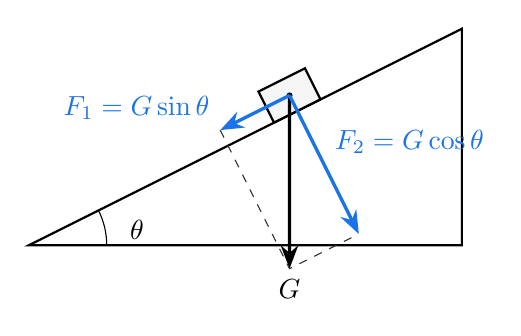
\begin{tikzpicture}[>=Stealth,scale=1.1]
  % 斜面：tanθ = 1/2，θ ≈ 26.57°，sinθ=0.4472，cosθ=0.8944
  \draw[thick] (0,0) -- (5,0) -- (5,2.5) -- cycle;
  \draw (0.9,0) arc (0:26.57:0.9) node at (1.25,0.18) {$\theta$};
  % 物块：绕中心旋转 θ，底边贴合斜面
  \draw[thick,fill=lightgray,rotate around={26.57:(3.01,1.73)}]
    (2.71,1.53) rectangle (3.31,1.93);
  \coordinate (C) at (3.01,1.73);
  \fill (C) circle (1pt);
  % 重力 G（长度取 2）
  \draw[->,very thick] (C) -- (3.01,-0.27) node[below] {$G$};
  % F1 = G sinθ（长度 0.894），方向 (-cosθ, -sinθ) → 偏移 (-0.8, -0.4)
  \draw[->,very thick,accent] (C) -- ($(C) + (-0.8,-0.4)$) node[above left] {$F_1=G\sin\theta$};
  % F2 = G cosθ（长度 1.789），方向 (sinθ, -cosθ) → 偏移 (0.8, -1.6)
  \draw[->,very thick,accent] (C) -- ($(C) + (0.8,-1.6)$) node[midway,above right] {$F_2=G\cos\theta$};
  % 分解的平行四边形（投影关系：F1 + F2 = G）
  \draw[dashed,darkgray] ($(C) + (-0.8,-0.4)$) -- (3.01,-0.27) -- ($(C) + (0.8,-1.6)$);
\end{tikzpicture}
\end{center}

斜面越陡（$\theta$ 越大），$\sin\theta$ 越大——为什么陡坡更难爬、更容易滑，这个分解就是答案。第 7 天它会成为牛顿第二定律的主战场。

\begin{exercise}[今日自测]
\begin{enumerate}
  \item 弹簧原长 10 cm，挂上 2 N 重物后长 14 cm。它的劲度系数是多少（N/m）？
  \item 两个大小都是 5 N 的力，夹角为 180°、120°、0° 时，合力各是多少？（夹 120° 时可用平行四边形几何性质）
  \item 用水平方向的力推桌子，桌子没动。此时静摩擦力是多少？它由什么决定？
\end{enumerate}
\end{exercise}

\newpage

% ═══ 第 6 天 ═══
\daytitle{第 6 天}{平衡的数学，与惯性的世界}

\textbf{核心问题}：物体什么时候保持现状？力之间的“账”怎么算平？

\subsection*{6.1 共点力平衡：矢量方程 F 合 = 0}

静止或做匀速直线运动的物体处于\textbf{平衡状态}。平衡不是因为“没有力”，而是因为\textbf{所有力的矢量和为零}：

\[
F_{\text{合}} = 0
\]

注意这是一个\textbf{矢量方程}：不是几个数字加起来为零，而是所有力按平行四边形定则首尾相接后恰好回到原点。一个有用的推论：\textbf{三个力平衡时，任意两个力的合力必与第三个力等大、反向}。

\begin{center}
\begin{tikzpicture}[>=Stealth,scale=1.1]
  \draw[thick] (-2.6,2.2) -- (2.6,2.2);
  \draw[thick,darkgray] (0,0) -- (-1.8,2.2) (0,0) -- (1.8,2.2);
  \fill (0,0) circle (1.8pt) node[below=6pt,right=2pt] {节点};
  \draw[->,very thick] (0,0) -- (-0.95,1.16) node[above left] {$T_1$};
  \draw[->,very thick] (0,0) -- (0.95,1.16) node[above right] {$T_2$};
  \draw[->,very thick,accent] (0,0) -- (0,-1.5) node[below] {$G$};
  \node[darkgray] at (0,2.45) {天花板};
\end{tikzpicture}
\end{center}

吊灯静止：两绳拉力 $T_1$、$T_2$ 的合力必然竖直向上、大小等于 $G$。会画这张图，就掌握了平衡问题的通用解法：\textbf{把力都画出来，让它们“加起来等于零”}。

\subsection*{6.2 牛顿第一定律：力不是维持运动的原因}

亚里士多德说“力是维持运动的原因”——推桌子桌子动，不推就停。伽利略的理想实验反驳了他：小球从斜面滚下，若水平面完全光滑，它将永远匀速滑下去；现实中停下，是摩擦力在捣蛋。\textbf{力是改变运动状态的原因，不是维持运动的原因。}

\begin{keyconcept}[惯性]
一切物体总保持匀速直线运动状态或静止状态，除非有力迫使它改变。这种性质叫\textbf{惯性}，\textbf{质量是惯性大小的唯一量度}——质量越大，运动状态越难改变。惯性不是力，不能说“物体受到惯性作用”。
\end{keyconcept}

\subsection*{6.3 牛顿第三定律：力总是成对出现}

你推墙，墙也在推你——所以你反而会向后滑。力的本质是\textbf{相互作用}：

\[
F = -F'
\]

作用力与反作用力大小相等、方向相反、作用在同一直线上——关键是：\textbf{作用在两个不同的物体上}。

\begin{keyconcept}[牛三 vs 二力平衡：一对最容易混淆的概念]
\begin{itemize}
  \item 作用力与反作用力：作用在\textbf{两个}物体上，永远同时存在，\textbf{不能}互相抵消；
  \item 平衡力：作用在\textbf{同一个}物体上，合力为零，可以抵消。
\end{itemize}
桌上的杯子：重力（地球拉杯子）与支持力（桌面托杯子）都作用在杯子上，是平衡力；杯子压桌面的力与桌面托杯子的力，才是作用力与反作用力。
\end{keyconcept}

\begin{exercise}[今日自测]
\begin{enumerate}
  \item 吊灯的两根绳对称，各与竖直方向成 30°。绳的拉力与重力 $G$ 是什么关系？（提示：两拉力的合力等于 $G$）
  \item 汽车加速前进时，汽车拉拖车的力大于拖车拉汽车的力。对吗？
  \item 用牛顿第一定律解释：公交车急刹车时，乘客为什么向前倾？
\end{enumerate}
\end{exercise}

\newpage
% ═══ 第 7 天 ═══
\daytitle{第 7 天}{$F = ma$：力学的发动机 + 一周总检验}

\textbf{核心问题}：力和运动，到底是谁决定谁？

\subsection*{7.1 牛顿第二定律：把前六天焊在一起}

前六天我们分头准备了两套语言：运动学（$x$、$v$、$a$）和力学（重力、弹力、摩擦力、合成与分解）。牛顿第二定律把它们焊成一个方程：

\[
F_{\text{合}} = ma
\]

\begin{keyconcept}[怎么读这个等式]
\begin{itemize}
  \item 因果关系：\textbf{合力是原因，加速度是结果}。有力就有加速度，立即产生；力消失，加速度立即消失。
  \item 方向关系：$a$ 的方向永远与 $F_{\text{合}}$ 相同（与 $v$ 无关）。
  \item 比例关系：同样的力，质量越大加速度越小——这就是“质量是惯性的量度”的定量表达。
  \item 单位：$1\ \text{N} = 1\ \text{kg}\cdot\text{m/s}^2$。牛顿这个单位就是为了让 $F=kma$ 里的 $k=1$ 而定义的。
\end{itemize}
\end{keyconcept}

现在回答第 5 天的问题：为什么 $G = mg$ 里的 $g$ 和自由落体的加速度是同一个数？因为自由落体时物体只受重力，由 $F_{\text{合}}=ma$ 得 $mg = ma$，所以 $a = g$——\textbf{任何质量的物体，自由落体加速度都相同}。质量在等式两边约掉了。这就是伽利略“轻重物体同时落地”的理论解释，也是 $g$ 两张面孔本就是同一张脸的原因。

\subsection*{7.2 力学单位制：用单位检查公式}

国际单位制（SI）有 7 个基本单位，力学只用其中 3 个：长度（m）、质量（kg）、时间（s），其余全是导出单位。给你一个立刻能用的技能：\textbf{任何公式，两边的单位必须相同}。

比如有人告诉你位移公式是 $x = vt + \frac{1}{2}at$，称一称单位：左边是 m；右边第一项是 m，第二项是 $\text{m/s}^2 \times \text{s} = \text{m/s}$。两边对不上，公式一定错（正确的是 $\frac{1}{2}at^2$）。考试时发现单位对不上，不用验算就知道写错了。

\subsection*{7.3 两类基本问题：必修一的完整闭环}

\begin{keyconcept}[牛顿第二定律的全部应用，只有两类]
\begin{itemize}
  \item \textbf{由运动求力}：运动学公式 $\rightarrow$ 求出 $a$ $\rightarrow$ 由 $F_{\text{合}}=ma$ 分析受力；
  \item \textbf{由受力求运动}：受力分析（合成/分解）$\rightarrow$ 求出 $F_{\text{合}}$ $\rightarrow$ 由 $a = F_{\text{合}}/m$ 回到运动学。
\end{itemize}
$a$ 是两岸之间的桥：运动学在此岸，受力分析在彼岸。
\end{keyconcept}

\subsection*{7.4 超重与失重：变的是“视重”，不是重力}

电梯加速上升时，你觉得身体变“沉”了。分析电梯里的人：受重力 $mg$ 向下、地板支持力 $N$ 向上，合力向上产生加速度：

\[
N - mg = ma \quad\Longrightarrow\quad N = m(g+a) > mg
\]

地板托你的力大于你的重力，你感觉变重了——\textbf{超重}。反过来加速下降时 $N = m(g-a) < mg$，是\textbf{失重}；若 $a=g$（自由下落），$N=0$，\textbf{完全失重}。

\begin{center}
\begin{tikzpicture}[>=Stealth,scale=1.0]
  % 电梯
  \draw[thick] (0,0) rectangle (2.8,3.4);
  % 人（简笔画）
  \draw[thick] (1.4,1.95) circle (0.22);
  \draw[thick] (1.4,1.73) -- (1.4,0.85);
  \draw[thick] (1.4,1.5) -- (1.05,1.15);
  \draw[thick] (1.4,1.5) -- (1.75,1.15);
  \draw[thick] (1.4,0.85) -- (1.12,0);
  \draw[thick] (1.4,0.85) -- (1.68,0);
  % 质心
  \fill (1.4,1.3) circle (1.8pt) node[left=4pt,darkgray] {\small 质心};
  % N 与 mg 都过质心；N > mg（超重）
  \draw[->,very thick,accent] (1.4,1.3) -- (1.4,3.05) node[pos=0.75,right=3pt] {$N$（变大）};
  \draw[->,very thick] (1.4,1.3) -- (1.4,0.12) node[midway,left=3pt] {$mg$};
  \draw[->,very thick,calcframe] (3.15,0.4) -- (3.15,1.6) node[right] {$a$ 向上};
  \node[darkgray] at (1.4,3.72) {电梯加速上升};
\end{tikzpicture}
\end{center}

要点：\textbf{重力 $mg$ 本身从没变过}，变的只是支持力（弹簧秤的读数，叫“视重”）。

\begin{exercise}[一周总检验]
\begin{enumerate}
  \item 质量 2 kg 的物体受到 10 N 的合力，加速度是多少？若它从静止开始运动 4 秒，位移是多少？
  \item 用单位检查：公式 $v^2 = 2ax$ 是否可能正确？（称两边的单位）
  \item 体重 60 kg 的人站在电梯里的体重秤上，电梯以 1 m/s$^2$ 加速下降（$g$ 取 10）。秤的读数是多少？
  \item 滑雪者沿 30° 雪坡下滑，把重力 $G=mg$ 沿斜面和垂直斜面分解，写出使滑雪者加速的那个分力。
  \item 用一句话向初中生解释：为什么轻重两个物体同时落地？
  \item 合上本讲义，画出“位置 → 速度 → 加速度”三级台阶，标出相邻两级之间各是什么运算。
\end{enumerate}
\end{exercise}

\newpage

% ═══ 参考答案 ═══
\section*{参考答案}
\addcontentsline{toc}{section}{参考答案}

\textbf{第 1 天}
\begin{enumerate}
  \item 不可以。研究自转时，地球上不同位置的运动不同（赤道快、两极慢），大小和形状恰恰是问题本身，不能忽略。
  \item 路程 400 m；位移 0（初末位置重合）。
  \item 位移 $+1$ m（即向东 1 m）；路程 7 m。
\end{enumerate}

\textbf{第 2 天}
\begin{enumerate}
  \item $\bar{v} = 100/10 = 10$ m/s。不能，平均速度只反映全程整体快慢，撞线瞬间的快慢要用瞬时速度描述。
  \item 图线越陡，斜率越大，瞬时速度越大——物体在加速。
  \item $\Delta t = 0$ 时 $\frac{\Delta x}{\Delta t} = \frac{0}{0}$ 没有意义；瞬时速度是 $\Delta t$ \textbf{趋近于} 0 时比值的极限，不是 $\Delta t$ 等于 0 时的值。
\end{enumerate}

\textbf{第 3 天}
\begin{enumerate}
  \item $a = \dfrac{20-10}{5} = 2$ m/s$^2$，方向与速度相同。
  \item 不一定。若物体速度为负（向负方向运动）且 $a = -2$ m/s$^2$，$a$ 与 $v$ 同号，物体在向负方向加速。判据是 $a$ 与 $v$ 同向加速、反向减速。
  \item 表示匀速直线运动；加速度为 0；$t$ 时间内的图线面积（矩形）$= v\,t$，即位移。
\end{enumerate}

\textbf{第 4 天}
\begin{enumerate}
  \item $v = 10 + 2\times5 = 20$ m/s；$x = 10\times5 + \frac{1}{2}\times2\times25 = 75$ m。
  \item $t = \sqrt{2h/g} = \sqrt{9} = 3$ s；$v = gt = 30$ m/s。
  \item $h = vt$ 只对匀速运动成立。自由落体是加速运动，应该用平均速度：$h = \bar{v}\,t = \frac{0+gt}{2}\cdot t = \frac{1}{2}gt^2$。他把末速度当成了全程的平均速度。
  \item 自由落体太快，当时的计时工具测不准；斜面“冲淡”了重力，使运动变慢、时间可测，再把规律外推到 90°。
\end{enumerate}

\textbf{第 5 天}
\begin{enumerate}
  \item 伸长量 $x = 4$ cm $= 0.04$ m，$k = F/x = 2/0.04 = 50$ N/m。
  \item 180°：0 N；120°：5 N（平行四边形为菱形，对角线等于边长）；0°：10 N。
  \item 静摩擦力等于所施的水平推力（二力平衡），它随推力变化、是被动力，上限是最大静摩擦力；不能套 $F_f=\mu F_N$。
\end{enumerate}

\textbf{第 6 天}
\begin{enumerate}
  \item 设每根绳拉力为 $T$，竖直方向的合力为 $2T\cos30° = G$，故 $T = \dfrac{G}{2\cos30°} = \dfrac{G}{\sqrt{3}} \approx 0.58\,G$。
  \item 不对。这是一对作用力与反作用力，任何时刻都大小相等——包括加速的时候。拖车加速是因为它受到的合力不为零，与牛三不矛盾。
  \item 乘客下半身随车减速，上半身由于惯性保持原来的速度继续向前，所以向前倾。车是参考系在变，不是有向前的“力”。
\end{enumerate}

\textbf{第 7 天（一周总检验）}
\begin{enumerate}
  \item $a = F/m = 5$ m/s$^2$；$x = \frac{1}{2}at^2 = \frac{1}{2}\times5\times16 = 40$ m。
  \item 左边单位为 m$^2$/s$^2$，右边为 $\text{m/s}^2 \times \text{m} = \text{m}^2/\text{s}^2$，两边一致——公式可能正确（单位一致只是必要条件）。
  \item 加速下降：$mg - N = ma$，$N = m(g-a) = 60\times9 = 540$ N，秤读数相当于 54 kg（失重）。
  \item 沿斜面分力 $F_1 = G\sin30° = 0.5\,mg$（使滑雪者加速）；垂直斜面分力 $F_2 = G\cos30° \approx 0.87\,mg$。
  \item 由 $F=ma$：重力 $mg$ 与质量成正比，代入 $a = F/m$ 后质量恰好约掉，所以一切物体自由落体加速度都是 $g$，与轻重无关。
  \item 位置 $\xrightarrow{\text{求导（变化率）}}$ 速度 $\xrightarrow{\text{求导（变化率）}}$ 加速度；反向：加速度 $\xrightarrow{\text{积分（累积）}}$ 速度 $\xrightarrow{\text{积分（累积）}}$ 位置。
\end{enumerate}

\vspace{1em}
\begin{keyconcept}[一周后，你应该能讲给别人听的五句话]
\begin{enumerate}
  \item 物理模型是“够用的简化”：能不能当质点，取决于问题，不取决于物体。
  \item 瞬时量都是极限：速度是位置的变化率，加速度是速度的变化率。
  \item $v$–$t$ 图：斜率是加速度，面积是位移；三个运动学公式都是这幅图的读法。
  \item 力是矢量，按平行四边形定则合成与分解；平衡就是 $F_{\text{合}}=0$。
  \item $F_{\text{合}}=ma$：力是改变运动的原因；知运动求力、知力求运动，都走 $a$ 这座桥。
\end{enumerate}
\end{keyconcept}

\end{document}
